\subsection{Qualitative Assessments for $\homcomp$}\label{sec:qual_comp}
\begin{table}[t!] 
    \centering
    \caption{Benchmark Results for Homomorphic $\geq$}
    % \vspace{0em}
        \begin{tabular}{cccccc}
            \toprule
            Precision & Methods & \multicolumn{2}{c}{Latency (ms)} & \multicolumn{2}{c}{Ciphertext (kB)} \\
                 %&         & (ms)      &         & (kB) & \\
            \midrule
             \multirow{4}*{4} & PEGASUS~\cite{pegasus} & 681 & $37.83\times$ & 8 & $2\times$ \\
             & SortingHat~\cite{sortinghat} & 444 & $24.67\times$ & 10 & $2.5\times$ \\
             & Liu \etal ~\cite{largeprecision} & 2040 & $113\times$ & 16 & $4\times$ \\
             % & Antonio\cite{revisiting} & 70 & $3.89\times$ & 5 & $1.25\times$ \\
             & \textbf{Ours} & 18 & $1\times$ & 4 & $1\times$ \\
             \midrule
            % \midrule
            %  \multirow{4}*{8} & Pegasus~\cite{pegasus} & 3027& $56.06\times$ & 8 & $2\times$ \\
            %  & SortingHat~\cite{sortinghat} & 1030 & $19.07\times$ & 19 & $4.75\times$ \\
            %  & Liu~\cite{largeprecision} & 4439 & $82.2\times$ & 16 & $4\times$ \\
            %  % & Antonio\cite{revisiting} & 138 & $2.56\times$ & 10 & $2.5\times$ \\
            %  & \NAME & \textbf{54} & $1\times$ & \textbf{4} & $1\times$ \\
            % \midrule
             \multirow{4}*{16} & PEGASUS~\cite{pegasus} & --- & --- & --- & --- \\
             & SortingHat~\cite{sortinghat} & 2186 & $8.13\times$ & 38 & $2.38\times$ \\
             & Liu \etal~\cite{largeprecision} & 7992 & $29.71\times$ & 16 & $1\times$ \\
             % & Antonio\cite{revisiting} & 277 & $1.03\times$ & 20 & $1.25\times$ \\
             & \textbf{Ours}  & 269 & $1\times$ & 16 & $1\times$ \\
            \midrule
             \multirow{4}*{32} & PEGASUS~\cite{pegasus} & --- & --- & --- & --- \\
             & SortingHat~\cite{sortinghat} & 4329 & $7.67\times$ & 76 & $4.75\times$ \\
             & Liu \etal~\cite{largeprecision} & --- & --- & --- & ---\\
             % & Antonio\cite{revisiting} & 202 & $1.22\times$ & 40 & $2.5\times$ \\
             & \textbf{Ours}  & 564 & $1\times$ & 16 & $1\times$ \\
            \bottomrule
        \end{tabular}
    \label{tab:combenchmark}
    {\footnotesize{$-$ means
    the method does not support such bits of precision.}}
    % \vspace{-3mm}
\end{table}

\begin{figure*}[t!]
   \begin{center}
    \begin{subfigure}[b]{0.3\textwidth}
    \centering
    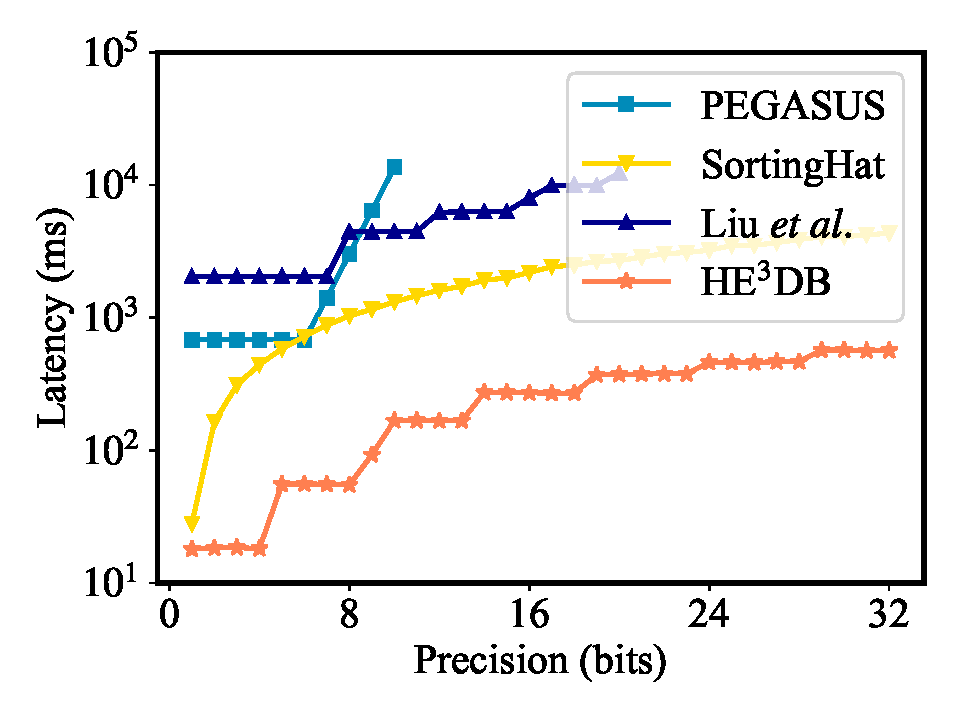
\includegraphics[width=\linewidth]{figure/com_micro_geq.pdf}
    % \vspace{-2em}
    \caption{Homomorphic $\geq$}
    \label{fig:homcompbench1}
    \end{subfigure}%
    \hfill
    \begin{subfigure}[b]{0.3\textwidth}
    \centering
    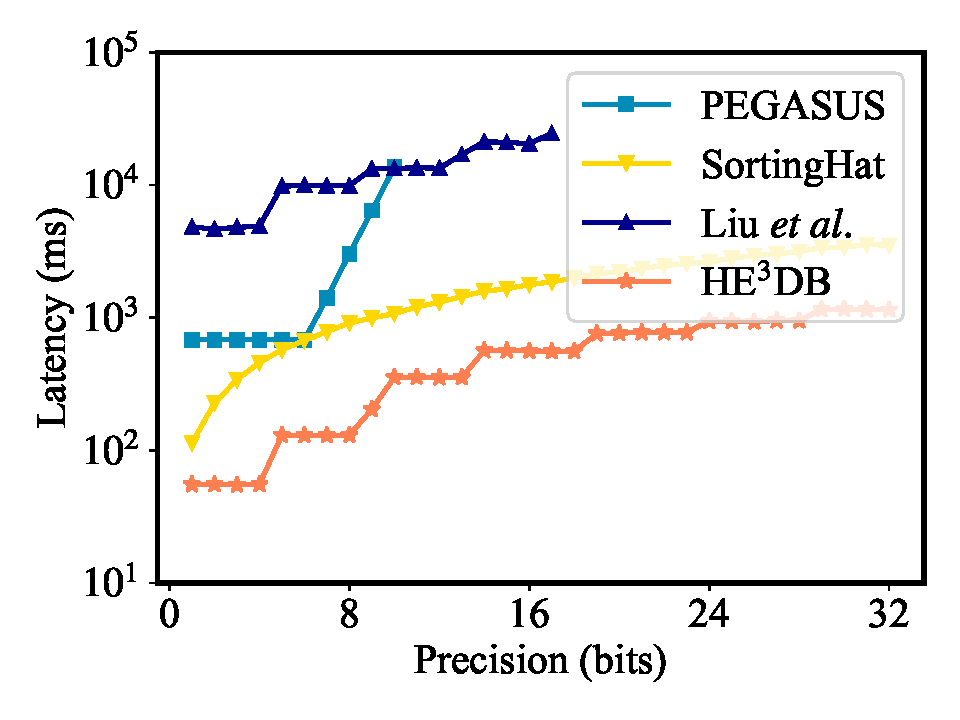
\includegraphics[width=\linewidth]{figure/com_micro_eq.pdf}
    % \vspace{-2em}
    \caption{Homomorphic $==$}
    \label{fig:homcompbench2}
    \end{subfigure}%
    \hfill
    \begin{subfigure}[b]{0.3\textwidth}
    \centering
    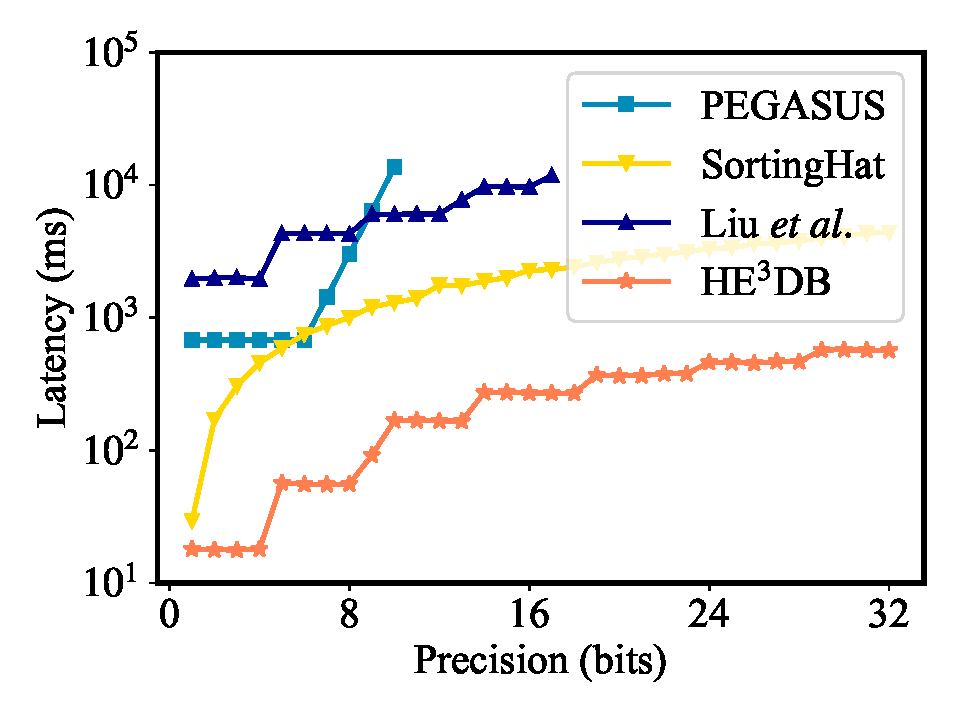
\includegraphics[width=\linewidth]{figure/com_micro_g.pdf}
    % \vspace{-2em}
    \caption{Homomorphic $>$}
    \label{fig:homcompbench3}
    \end{subfigure}%
   
   \end{center}
    % \vspace{-0.5em}
      \caption{Benchmark results for homomorphic comparison for the 
      $\geq, ==, >$ comparison operators 
       with varying bit precision.}
       \Description{Benchmark results for homomorphic comparison for the 
      $\geq, ==, >$ comparison operators 
       with varying bit precision. 
       The horizontal axis is the bits of precision, and the vertical axis is the latency. 
       Our results achieve competitive performance across different
       comparison operators}
   \label{fig: homcompbench}
   % \vspace{-0.5em}
\end{figure*}
Since $\homcomp$ is one of the key homomorphic operators proposed
in this work, we first compare our $\homcomp$ with other related 
homomorphic comparison algorithms qualitatively, and
defer quantitative results to \cref{eva: microbenchmarks}.
% have their own advantages and 
% method selection depends on the application.
In the beginning, we note that approaches like PEGASUS~\cite{pegasus} and the method 
proposed by Liu \etal~\cite{largeprecision} focus on evaluating
arbitrary logic
functions over homomorphically encrypted ciphertext,
%by proposing efficient or large-precision PBS algorithms
while \NAME concentrates on the design of a homomorphic comparison algorithm.
Therefore, our method achieves better comparison accuracy as well
as efficiency than~\cite{pegasus, largeprecision}. In contrast
to general methods, 
SortingHat~\cite{sortinghat} proposes an efficient plaintext-ciphertext 
comparison algorithm, where one of the inputs to the comparison
is known to the server. Nonetheless, under an SDO setting,
SortingHat shows poor efficiency for ciphertext-ciphertext
comparisons. The method of Antonio \etal~\cite{revisiting} 
encrypts the input in a bit-wise manner, where binary circuits
can be used to construct fast and high-precision
homomorphic comparison. However, due to the encoding scheme, 
the algorithm in~\cite{revisiting} produces
a comparison result of $\{-1,0,1\}$, which cannot be used as
filters for subsequent aggregations.
Similarly, the polynomial approximation technique proposed by 
Cheon \etal~\cite{ckkscomparison} cannot support encrypted 
aggregations over results from equality tests \texttt{==}, for the approximate polynomial evaluates
to $1/2$ when the inputs are equal.
On the other hand, some works also suggest to encrypt all database items bit-by-bit in a
SIMD manner to accelerate the comparison process~\cite{aphadb, khedr2015shield}.
%due to the noise growth of RLWE ciphertext 
%as we discussed in \cref{pre:he_type}.
However, in such approaches, the client encrypts the 
entire database using an {\it{a-priori}} fixed-set parameters 
that are dependent on
the pre-defined maximum predicate depth. As a result,
any query that requires more predicate evaluations than the
pre-defined maximum depth cannot be directly
evaluated. Here, the only solution is to re-encrypt
entire database using a new set of encryption parameters, which
can be too costly for SDO clients.
%respectively representing the \texttt{<}, \texttt{==} and \texttt{>}.
% However, Antonio's approach~\cite{revisiting} does not support 
% the encrypted database scenarios as the result of the comparison 
% could not perform logic gate operation between various predicates.

% Different from the above approaches, a line of works investigate
% how to utilize polynomial approximations 
% to evaluate homomorphic comparisons over RLWE 
% ciphertexts~\cite{ckkscomparison}. 
% By leveraging
% the SIMD capability of RLWE ciphertext,
% such algorithm can achieve fast evaluation speed when processing
% a large number of parallel comparisons.
% Nonetheless, both of their methods do not meet the elasticity requirement.


% However, changing encryption parameters in~\cite{aphadb} requires the re-encryption
% of the entire database, which can bring about severe communcation 
% burdens on the client side in practice.
% encrypted queries that are more complicated than such depth.
% We list the qualitative comparisons between existing methods and 
% provide quantitative comparisons in \cref{eva: microbenchmarks}.

% Since not all of the methods summarized
% in \cref{eva: microbenchmarks} have the same design objective,
